% Activate the following line by filling in the right side. If for example the name of the root file is Main.tex, write
% "...root = Main.tex" if the chapter file is in the same directory, and "...root = ../Main.tex" if the chapter is in a subdirectory.
 
%!TEX root =  TNTinderSee.tex

Sedimentproben haben wir an den Stellen entnommen, an denen ungewöhnliche Erhebungen am Meeresboden zu finden waren. 
Dazu sind wir mit dem ROV bis auf den Meeresboden gefahren, um mit der Probenschaufel dort von der Bodenoberfläche eine Bodenprobe an die Oberfläche zu bringen. Dort wurde die Probe in einem Probenbeutel zur späteren Analyse gesichert.

\begin{figure}[htb]
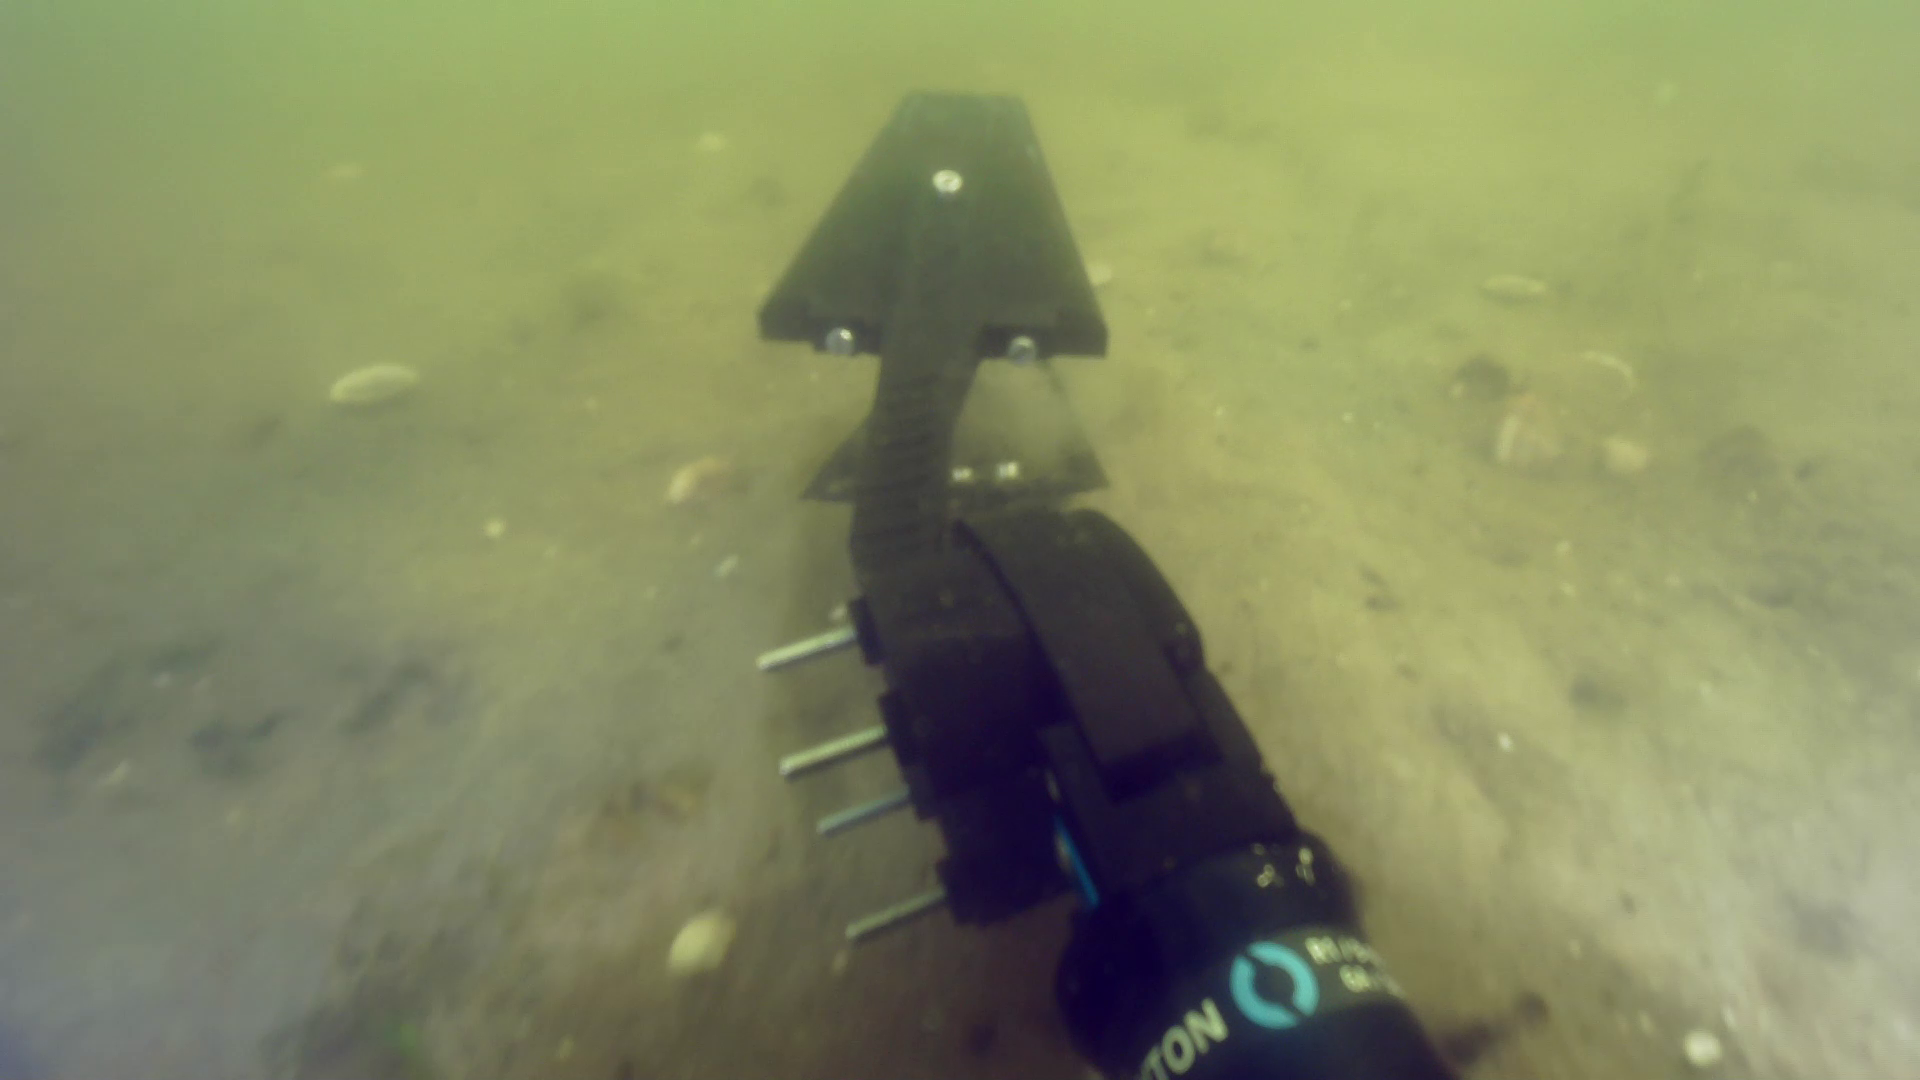
\includegraphics[height=\textheight,%
                   width=\textwidth,%
                   keepaspectratio]{Bilder/ROV/Sedimentprobe3.png}
\caption{ROV bei der Sedimentprobenentnahme. Die Probenschaufel ist eine Eigenentwicklung}
\end{figure}